\documentclass[a4paper,11pt]{report}
\usepackage[utf8]{vietnam}
\usepackage[dvipsnames,svgnames,table]{xcolor}
\usepackage{graphicx}
\usepackage{multirow}
\usepackage{multicol}
\usepackage{fancybox}
\usepackage{xcolor}
\definecolor{dkgreen}{rgb}{0,0.6,0}
\definecolor{gray}{rgb}{0.5,0.5,0.5}
\definecolor{mauve}{rgb}{0.58,0,0.82}
\definecolor{hilight}{RGB}{22,155,104}
  
\definecolor{Xanh}{rgb}{0,0.5,1}
\definecolor{Do}{rgb}{1,0.25,0}
\definecolor{Vang}{rgb}{1,1,0}
\definecolor{Datroi}{rgb}{0,0,1}

\usepackage{amsmath}
\usepackage{amssymb}
\usepackage[linesnumbered,ruled]{algorithm2e}
\usepackage[colorlinks = true,
            linkcolor = black,
            urlcolor  = blue,
            citecolor = blue,
            anchorcolor = blue]{hyperref}
\usepackage{longtable}
\usepackage{listings}
\newcommand{\bi}{\begin{itemize}}
\newcommand{\ei}{\end{itemize}}
\lstset{language=C++,
   %keywords={break,case,catch,continue,else,elseif,end,for,function,
   %   global,if,otherwise,persistent,return,switch,try,while},
   basicstyle=\ttfamily \fontsize{10}{12}\selectfont,   
   numbers=left,
   frame=lrtb
  }

\usepackage[left=3cm, right=2.00cm, top=2.00cm, bottom=2.00cm]{geometry}
\begin{document}
\thispagestyle{empty}
\thisfancypage{
\setlength{\fboxrule}{1pt}
\doublebox}{}
\begin{center}
{\fontsize{16}{19}\fontfamily{cmr}\selectfont TRƯỜNG ĐẠI HỌC BÁCH KHOA HÀ NỘI\\
VIỆN CÔNG NGHỆ THÔNG TIN VÀ TRUYỀN THÔNG}\\
\textbf{------------*******---------------}\\[1cm]

\includegraphics[scale=0.13]{hust.jpg}\\[1.3cm]

{\fontsize{32}{43}\fontfamily{cmr}\selectfont BÁO CÁO}\\[0.1cm]
{\fontsize{38}{45}\fontfamily{cmr}\fontseries{b}\selectfont MÔN HỌC}\\[0.2cm]
{\fontsize{19}{20}\fontfamily{phv}\selectfont Khai phá Web}\\[1cm]
{\fontsize{17}{24}\fontfamily{cmr}\selectfont Đề tài:}\\[1cm]
{\fontsize{17}{24}\fontfamily{cmr}\selectfont Cài đặt thử nghiệm một số phương pháp gợi ý phim }\\[2cm]
\end{center}
\hspace{1cm}\fontsize{14}{16}\fontfamily{cmr}\selectfont \textbf{Sinh viên thực hiện:}
\begin{longtable}{l c c }
Họ và Tên & MSSV &    Mã học phần \\[0.5cm]
Đặng Quang Trung &    20134145 & IT4868\\
Trần Bá Thiết & 20133736 &IT4868
\end{longtable}
\hspace{0.3cm}\fontsize{14}{16}\fontfamily{cmr}\selectfont \textbf{Giáo viên hướng dẫn:} TS. Nguyễn Kiêm Hiếu\\[1.0cm]
\begin{center}
\fontsize{16}{19}\fontfamily{cmr}\selectfont Hà Nội 10-05-2017
\end{center} 
\tableofcontents
\chapter*{Lời mở đầu}
\addcontentsline{toc}{chapter}{Lời mở đầu}
Sự phát triển của công nghệ thông tin và việc ứng dụng công nghệ thông tin trong nhiều
lĩnh vực của đời sống, kinh tế xã hội trong nhiều năm qua cũng đồng nghĩa với lượng dữ
liệu đã được các cơ quan thu thập và lưu trữ ngày một tích luỹ nhiều lên. Họ lưu trữ các
dữ liệu này vì cho rằng trong nó ẩn chứa những giá trị nhất định nào đó. Mặt khác, trong
môi trường cạnh tranh, người ta ngày càng cần có nhiều thông tin với tốc độ nhanh để trợ
giúp việc ra quyết định và ngày càng có nhiều câu hỏi mang tính chất định tính cần phải
trả lời dựa trên một khối lượng dữ liệu khổng lồ đã có. Với những lý do như vậy, các
phương pháp quản trị và khai thác cơ sở dữ liệu truyền thống ngày càng không đáp ứng
được thực tế đã làm phát triển một khuynh hướng kỹ thuật mới đó là Kỹ thuật phát hiện
tri thức và khai phá dữ liệu. \\ \\ 
Khai phá dữ liệu đã và đang được nghiên cứu, ứng dụng trong nhiều lĩnh vực khác nhau
ở các nước trên thế giới, tại Việt Nam kỹ thuật này tương đối còn mới mẻ tuy nhiên cũng
đang được nghiên cứu và dần đưa vào ứng dụng. Khai phá dữ liệu là một bước trong qui
trình phát hiện tri thức gồm có các thuật toán khai thác dữ liệu chuyên dùng dưới một số
qui định về hiệu quả tính toán chấp nhận được để tìm ra các mẫu hoặc các mô hình trong
dữ liệu. Nói một cách khác, mục đích của phát hiện tri thức và khai phá dữ liệu chính là
tìm ra các mẫu và/hoặc các mô hình đang tồn tại trong các cơ sở dữ liệu nhưng vẫn còn bị
che khuất bởi hàng núi dữ liệu. \\ \\ 
Trong bài viết này, em sẽ trình bày một cách tổng quan về Kỹ thuật khai phá dữ liệu.
Trên cơ sở đó đưa ra một bài toán Gợi ý phim cho người dùng của một hệ thống và giải
quyết bài toán bằng phương pháp Collaborative Filtering. 

\chapter*{Lời cảm ơn}
\addcontentsline{toc}{chapter}{Lời cảm ơn}
Chúng em xin chân thành cảm ơn thầy Nguyễn Kiêm Hiếu đã cung cấp cho chúng em những kiến thức vô cứng bổ ích khi chúng em bắt đầu tìm hiểu về môn học khai phá dữ liệu web cũng như đã giúp đỡ chúng em rất nhiều trong quá trình thực nghiệm và viết bản báo cáo này.
\chapter{Mô tả bài toán}
\section{Giới thiệu}
Hằng ngày chúng ta có các ý kiến về những thứ chúng ta thích hoặc không thích và thậm chí là không quan tâm đến nó. Ví dụ như bạn xem một chương trình truyền hình trên TV, bạn cảm thấy chương trình rất hay và hài hước hoặc thấy nó nhàm chán hay bạn không tìm thấy chương trình đó ở tất cả mọi kênh.Hoặc chương trình đó diễn ra mà chúng ta không để ý.\\ \\
Các sở thích của mỗi người là khác nhau, nhưng chúng ta tạo ra các dạng mẫu người dùng. Mọi người có xu hướng thích những thứ tương tự như những thứ mà họ thích. Bởi vì nếu tôi thích bộ phim Matrix, bạn có thế đoán là tôi cũng muốn xem báo cáo về  Minority, những cái này chủ yếu cùng một thể loại hành động và khoa học viễn tưởng. Tương tự như vậy moi người cũng có khuynh hướng thích những thứ mà người tương tự thích. Gợi ý là đề xuất tất cả về dự đoán những điều thích và không thích này và sử dụng chúng để khám phá những điều mới và đáng mong bạn chưa biết về chúng.
\section{Gơi ý là gì?}
Trong báo cáo này sẽ nói về một số cách mọi người đưa ra các khuyến nghị và khám phá các điều mới. Có một vài chiến lược sử dụng để tạo ra các khuyến nghị: Một là có thể đựa vào những người có cùng thị hiếu sở thích. Hoặc phương pháp khác sẽ tìm ra những thứ giống như những gì chúng ta đã thích.\\ \\
Ở đây bài báo cáo sẽ trình bày 2 phương pháp dùng để khuyến nghị đó là học cộng tác( Collaborative Filtering ) và nhân tố ẩn ( Lantent factors ).
\newpage
\section{Mô tả bộ dữ liệu}
Trong bài báo cáo này cài đặt thử nghiệm với 2 bộ dữ liệu:
\begin{itemize}
\item[•] ml-100k, bộ dữ liệu này có chứa:
\begin{itemize}
\item[-] Bộ 100,000 ratings (1-5) của 943 users trên 1682 bộ phim.
\item[-] Mỗi user đánh giá ít nhất 20 bộ phim.
\item[-] Dữ liệu rating chứa trong 2 files là u.data và u.item
\end{itemize}
\item[•] ml-1m, bô dữ liệu này có chứa:
\begin{itemize}
\item[-] 100,000,54 ratings (1-5) của 71567 users trên 10681 bộ phim.
\item[-] Mỗi user đánh giá ít nhất 20 bộ phim.
\item[-] Dữ liệu rating chứa trong 3 files là moives.dat , ratings.dat và tags.dat
\end{itemize}
\end{itemize}
Bộ dư trện có thể ở: \href{https://grouplens.org/datasets/movielens/}{moivelens}. Bộ dữ liệu trên đã được trường đại học Minnesota và bất kì nhà nghiên cứu nào có thể đảm bảo tính đúng đắn của dữ liệu, tính phù hợp của nó cho bất kỳ mục đích cụ thể nào, hoặc tính hợp lệ của các kết quả dựa trên việc sử dụng bộ dữ liệu.của nó cho bất kỳ mục đích cụ thể nào, hoặc tính hợp lệ của các kết quả dựa trên việc sử dụng bộ dữ liệu.\\ \\
Cấu trúc nội dung và cách sử dụng các files trong bộ dữ liệu.
\subsection{User Ids}
Người sử dụng của Movielens đã được lựa chọn ngẫu nhiên để đưa vào. Id của họ đã được ẩn danh. 
\subsection{Cấu trúc file Ratings}
Tất cả các rating đều được chứa trong tệp xếp ratings.dat. Mỗi dòng của tệp này đại diện cho một rating của một bộ phim của một người dùng và có định dạng sau:
\begin{itemize}
\item[] UserID::MovieID::Rating::Timestamp
\end{itemize}
Rating được thực hiện theo thang điểm 5 sao với số gia tăng nửa sao. Mẫu thời gian biểu thị bằng giây từ nửa đêm(UTC) ngày 1 tháng 1 năm 1970.
\newpage
\subsection{Cấu trúc file Moives}
Thông tin phim có trong tệp moives.dat. Mỗi dòng của tệp này đại diện cho một bộ phim và có định dạng sau:
\begin{itemize}
\item[] MovieID::Title::Genres
\end{itemize}
MovieID là id MovieLens thực. Tiêu đề phim, theo chính sách, phải được nhập giống với những bài tìm thấy trong IMDB, kể cả năm phát hành. Tuy nhiên, chúng được nhập bằng tay, do đó, lỗi và không nhất quán có thể tồn tại. Các thể loại là một danh sách được cách ly bằng đường ống, và được chọn từ các loại sau: \textbf{Action, Adventure, Animation, Children's, Comedy, Crime, Documentary, Drama, Fantasy, Film-Noir, Horror, Musical, Mystery, Romance, Sci-Fi, Thriller, War, Western}
\chapter{Collaborative Filtering}
\section{Ý tưởng của phương pháp}
\begin{figure}[h]
\begin{center}
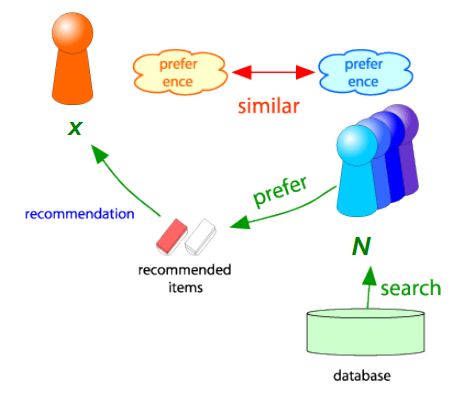
\includegraphics[width =0.6 \textwidth]{CF.png}
\end{center}
\end{figure}
\begin{itemize}
\item[•] quan sát một người dùng x.
\item[•] Tìm tập N các người dùng khác cũng rating giống như các ratings của người dùng x.
\item[•] Ước lượng các ratings của người dùng x dựa trên các ratings của những người trong tập N.
\end{itemize}
\section{Tìm tập người sử dụng tương đồng}
Mỗi người dùng sẽ có một vector ratings biểu diễn đánh giá của người đó về các bộ phim mà họ đã xem ví du: $r_x = [*,\_,\_,*,***]$. Để tìm sử tương đồng giữa các người sử dụng với nhau chúng ta có thể sử dụng một số độ đo như:
\begin{itemize}
\item[•] Độ đo tương đồng jaccard
\begin{itemize}
\item[-] Vấn đề: khi sử dụng độ đo jaccard nó sẽ không quan tâm các giá trị ratings của người dùng
\end{itemize}
\item[•] Độ đo tương đồng Cosine
\begin{itemize}
\item[-] $sim(x,y) = \cos(\vec{r}_x , \vec{r}_y) = \frac{\vec{r}_x.\vec{r}_y}{\parallel \vec{r}_x \parallel . \parallel \vec{r}_y \parallel}$
\item[-] Vấn đề: khắc phục được nhược điểm của jaccard nhưng lại bỏ qua các ratings không tốt(người dùng đánh giá thấp bộ phim đó)
\end{itemize}
\item[•] Sử dụng hệ số tương phản cá nhân
\begin{itemize}
\item[-] $S_{xy}$ là tập các bộ phim được rating bởi x và y.
\small{
\item[-] $sim(x,,y) = \sum s\in S\downarrow xy \uparrow (r\downarrow xs - r\downarrow x)r\downarrow ys - r\downarrow y)/\sqrt{\sum s\in S\downarrow xy \uparrow (r\downarrow xs - r\downarrow x)\uparrow 2}$
}
\end{itemize}
\end{itemize}
Khi cài đặt thư nghiêm sử dụng độ đo cosine. Có ví dụ sau:
\begin{center}
\begin{longtable}{c|ccccccc}
 & HP1 & HP2 & HP3 & TW & SW1 & SW2 & SW3 \\
 \hline
A & 4 & & & 5 & 1 & \\
B & 5 & 5 & 4 &   &  \\
C &  &   &  & 2 & 5 & 5\\
D &  & 3 &  &  &  &  & 3 \\
\end{longtable}
\end{center}
\begin{itemize}
\item Ta muốn: $sim(A,B) > sim(A,C)$
\item Độ đo jaccard: 1/5 < 2/4
\item Độ đo Cosine: 0.386 > 0.322
\begin{itemize}
\item[-] Mất đi sự xem xét các ratings bị người dùng đánh giá thấp.
\item[-] Để giải quyết vấn đề này chúng ta sẽ trừ đi trung bình rating của hàng.
\end{itemize}
\end{itemize}
\begin{center}
\begin{longtable}{c|ccccccc}
 & HP1 & HP2 & HP3 & TW & SW1 & SW2 & SW3 \\
 \hline
A & 2/3 & & & 5/3 & -7/3 & \\
B & 1/3 & 1/3 & -2/3 &   &  \\
C &  &   &  & -5/3 & 1/3 & 4/3\\
D &  & 0 &  &  &  &  & 0 \\
\end{longtable}
\end{center}
Khi đó: $sim(A,B) = 0.092 > -0.559$
\section{Dự đoán rating}
Từ tập số liệu gợi ý ta có:
\begin{itemize}
\item[•] Cho $r_x$ là vector người dùng(những bộ phim mà x đã đánh giá có giá trị từ 1-5 còn chưa có giá trị là 0).
\item[•] Cho N là tập k người dùng có sở thích gần giống với x( x là người mà cần gợi ý phim)
\end{itemize}
Đánh giá theo cách nhìn Item-Item:
\begin{itemize}
\item[•] Cho bộ phim i, tìm các bộ phim khác tương tự như i.
\item[•] Ước lượng ratings cho bộ phim i dựa trên ratings của các bộ phim tương tự.
\item[•] Sử dụng Công thức sau:
\end{itemize}

\begin{center}
\textbf{\huge{
$r_{xi} = \frac{\sum_{j\in N(r,x)}s_{ij}.r_{xj}}{2}$
}}
\end{center}
Trong đó:
\begin{itemize}
\item[-] $s_{ij}$\ldots là độ tương đồng giữa i và j.
\item[-] $r_{xj}$\ldots là rating của x với bộ phim j.
\item[-] $N(i;x)$\ldots tập các bộ phim được rating bởi x.
\end{itemize}
\section{Dự đoán rating trong thực tế}
Trong thực tế để có được một dự đoán chính xác hơn chúng ta thêm cả ước lượng độ lệch cho rating của người dùng với bộ phim.
\subsection{Tổng quát:}
\begin{itemize}
\item[•] Rating trung bình của phim: 3.7 sao.
\item[•] Bộ phim Sixth Sense cao hơn trung bình là 0.5 sao.
\item[•] Trung bình các đánh giá của Joe về phim thấp hơn 0.2 sao.
\begin{itemize}
\item[] $\rightarrow$ Uớc lượng: bộ phim Sixth Sense Joe sẽ đánh giá là 4 sao.
\end{itemize}
\end{itemize}
\subsection{Hàng xóm lân cận(CF/NN):}
\begin{itemize}
\item[•] Joe không thích bộ phim Signs
\item[•] $\rightarrow$ Ước lượng cuối cùng cho bộ phim Sixth Sense là 3.8 sao.
\end{itemize}
Vì thế trong thực tế chúng ta sẽ có được ước lượng tốt nhất theo mô hình sai lệch sau:
\newpage
\begin{center}
\huge{
$\hat{r_{xi}} = b_{xi} + \frac{\sum_{j\in N(i;x)}s_{ị}.(r_{xj} - b_{xj})}{\sum_{j\in N(i;x)}s_{ị} }$
}
\end{center}
Với $b_{xi} = \mu + b_x + b_i$ là độ lệch cơ sở của người dùng x khi đánh giá bộ phim i. Trong đó:
\begin{itemize}
\item[-] $\mu$ là rating trung bình của tất cả người dùng.
\item[-] $b_x$ là độ lệch của người dùng x.
\begin{itemize}
\item[] $b_x = avg(x) - \mu $.
\end{itemize}
\item[-] $b_i$ là độ lệch của bộ phim i.
\begin{itemize}
\item[] $b_i = avg(i) - \mu $.
\end{itemize}
\end{itemize}
\section{Ưu và nhược điểm của phương pháp}
\subsection{Ưu điểm:}
\begin{itemize}
\item[•] Làm việc với bất kì loại phim không cần quan tâm đến đặc điểm lựa chọn.
\item[•] Dễ dàng cài đặt. 
\end{itemize}
\subsection{Nhược điểm:}
\begin{itemize}
\item[•] Khi chạy cần có đủ user trên hệ thống.
\item[•] Tính thưa:
\begin{itemize}
\item[-] dữ liệu là một ma trận thưa.
\item[-] Khó có thể tìm thất những người dùng có ratings tương tự nhau.
\end{itemize}
\item[•] Không thể gợi ý những phim mà chưa được ai đánh giá trước đó.
\end{itemize}
\chapter{Latent Factor Models}
\section{Ý tưởng của phương pháp}
Trong thức tế mỗi người dùng sẽ có những sở thích riêng của mình ví dụ như có người thích phim tình cảm, lãng mạn có người thích phim hành động, khoa học viễn tưởng, \ldots . Những sở thích đó được coi là một nhân tố ẩn của mỗi người dùng.
\begin{figure}[h]
\begin{center}
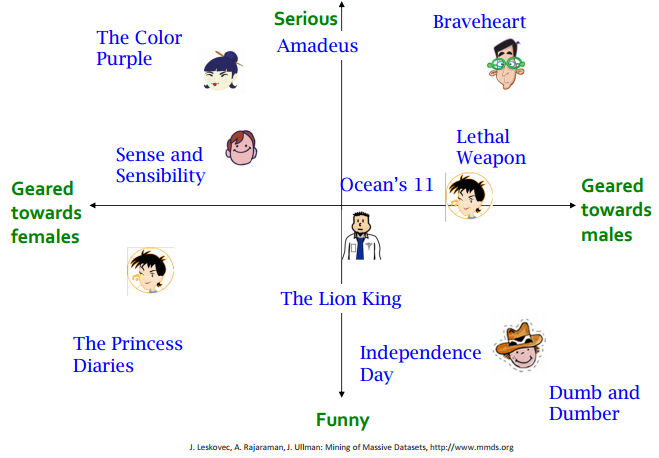
\includegraphics[scale=0.6]{LF.png}
\caption{hình ảnh về factors}
\end{center}
\end{figure}
\begin{itemize}
\item[•] Các ratings chịu ảnh hưởng sâu sắc bởi một bộ các nhân tố(factor) rất cụ thể cho miền.
\item[•] Một số các factors là rất khó quan sát được và khó ước lượng sự tác động của chúng đối với ratings của người dùng.
\item[•] Mục tiêu là suy luận những nhân tố tiềm ẩn từ dữ liệu đánh giá bằng cách sử dụng các kỹ thuật toán học.
\end{itemize}
\section{SVD}
SVD là một phương pháp trong toán học dùng để giảm chiều ma trận làm sao cho sự mất mát thông tin là ít nhất. \\  \\
Giả sử ta có ma trận $A_{n*p}$ ta có:
\begin{center}
\huge{
$A_{n*p} = U_{n*n}S_{n*p}V^{T}_{p*p}$
}
\end{center}
Trong đó:
\begin{itemize}
\item[-] U là ma trận vói các cột là các vector trái.
\item[-] S là ma trận cùng kích thước như A giá trị đợn là đường chéo.
\item[-] $V^T$ có các hàng là cá vector đơn phải 
\end{itemize}
SVD thể hiện sự mở rộng của dữ liệu ban đầu trong một hệ tọa độ nơi ma trận hiệp phương sai là đường chéo.
\begin{figure}[h]
\begin{center}
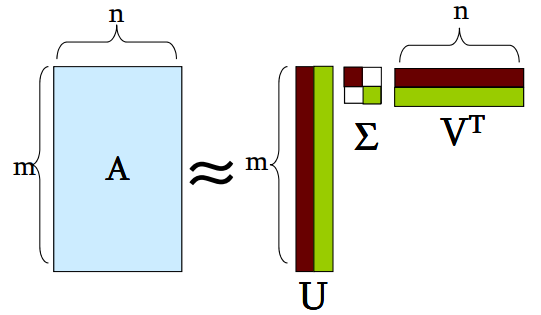
\includegraphics[scale=0.8]{svd.png}
\end{center}
\caption{Hình ảnh minh họa svd}
\end{figure}
\section{Dự đoán rating}
Để dự đoán rating người dùng ban đầu ta có ma trận người dùng sử dụng svd để giảm chiều mà trận và phân tách thành ma trận trận là mat trận người dùng và ma trận user
\begin{figure}
\begin{center}
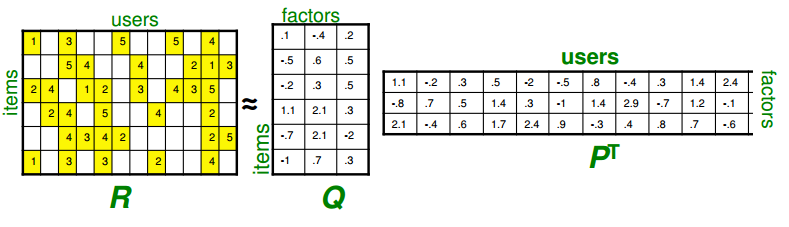
\includegraphics[scale=0.8]{svd1.png}
\caption{ma trận sau khi giảm chiều sử dụng svd}
\end{center}
\end{figure}
\newpage
Trong đó:
\begin{itemize}
\item[•] A = R là ma trận người dùng ban đầu.
\item[•] Q là ma trận nhân tố của phim.
\item[•] $P^T$ là ma trận nhân tố của người dùng.
\begin{itemize}
\item[] $P^T = \sum V^T$
\end{itemize}
\end{itemize}
Để dự đoán rating của người dùng x cho một bộ phim ra chỉ cần tính:
\begin{center}
$\hat{r_{xi}} = q_i.p_x = \sum_fq_{if}.p_{xf}$
\end{center}
Trong đó:
\begin{itemize}
\item[-] $q_i$ là hàng i của ma trận Q.
\item[-] $p_x$ là cột x của ma trận P.
\item[-] f là số factors(hay độ dài vector của hàng i và cột x).
\end{itemize}
\section{Tối thiểu hóa lỗi RMSE}
Như đã biết SVD đã tối thiếu hóa lỗi trên toàn ma trận để ít mất mát thông tin nhất.Chúng ta có thể xây dựng lại hàm lỗi:
\begin{center}
\LARGE{
$min_{U,V,\sum}\sum(A_{ij} - [U \sum V_{T}]_{ij})^2$
}
\end{center}
Bởi vì ma trận người dùng là thưa nên có rất nhiều rating bằng không vì thế cần tối thiểu RMSE cho các dữ liệu không nhìn thấy. \\ 
\textbf{Ý tưởng:} tối thiểu hóa RMSE trên tập dữ liệu.
\begin{itemize}
\item[•] k (số nhân tố) bắt tất cả các đặc điểm người dùng.
\item[•] Nhưng RMSE trên bộ test bắt đầu với k > 2
\end{itemize}
\textbf{Vấn đề Overfitting:}
\begin{itemize}
\item[•] Với quá nhiều tham số tự do thì mô hình sẽ trở nên fitting.
\item[•] Để giải quyết vấn đề overfitting không cho P,Q quá tự do học.
\end{itemize}
\begin{center}
\begin{displaymath}
\displaystyle\min_{P,Q} \sum_{training}\underbrace{(r_{xi} - q_ip_x)^2}_{error} + [\lambda_1\underbrace{\sum_{x}\Vert p_x \Vert^{2} + \lambda_2\sum_i\Vert q_i \Vert^2}_{length}]
\end{displaymath}
\end{center}
Ở đây:
\begin{itemize}
\item[-] $\lambda_1$ và $ \lambda_2$ là các hệ số phạt của p và q
\item[-] Sử dụng gradient descent để tối thiểu hóa lỗi của hàm trên
\end{itemize}
\section{Mở rộng mô hình latent với độ lệch}
Để có một ước lượng chính xác hơn trong thực tế chúng ta có thể thêm vào độ lệch rating của người dùng và của phim.Khi đó ta có ratings của người dùng x sẽ đánh giá bộ phim i như sau:
\begin{center}
$r_{xi} = \underbrace{\mu}_{overall mean rating} + \underbrace{b_{x}}_{bias for user x} + \underbrace{b_{i}}_{bias for moive i} + q_{x}.p_i$
\end{center}
\subsection{Vấn đề tối ưu hóa lỗi và overfitting:}
Giải pháp:
\begin{flushleft}
\begin{displaymath}
\displaystyle \min_{Q,P} \sum_{(x,i)\in R}(r_{xi} - (\mu + b_x + b_i + q_i.p_x))^2
\end{displaymath}
\end{flushleft}
\begin{center}
\begin{displaymath}
\displaystyle
+ (\lambda_1\sum_{i}\Vert q_i \Vert^{2} + \lambda_2\sum_x\Vert p_x \Vert^2 + \lambda_3\sum_x\Vert b_x \Vert^2 + \lambda_4\sum_i\Vert b_i \Vert^2)
\end{displaymath}
\end{center}
Trong đó:
\begin{itemize}
\item[-] $\lambda_1,\lambda_2,\lambda_3,\lambda_4$ là các hệ số phạt.
\begin{itemize}
\item[+] Để đơn giản ở đây tất cả dùng chung $\lambda$
\end{itemize}
\item[-] $b_i,b_x$ là độ lệch của moive và người dùng.
\item[-] $\mu$ là raitng trung bình của ma trận người dùng.
\item[-] $q_i,p_x$ là các vector hàng và cột của ma trận Q,P.
\end{itemize}
\newpage
\subsection{Sử dụng Stochastic Gradient Descent}
Xét người dùng x và bộ phim i. Giả sử đạo hàm riêng phần theo $q_{if}$ Ta có:
\begin{displaymath}
\triangledown Q = [\triangledown q_{if}] \  and  \ 
\triangledown q_{if} = \sum_{x,i} - 2(r_{xi} - q_ip_x)p_xf + 2\lambda q_{if}
\end{displaymath}
\begin{itemize}
\item Ở đây $q_if$ nhân tố f của hàng $q_i$ của matrix Q
\end{itemize}
Cập nhật trọng số cho Q theo Stochastic Gradient Descent
\begin{displaymath}
Q = Q - \mu \triangledown Q(r_{xi})
\end{displaymath}
Cập nhật tổng quát:
\begin{itemize}
\item[] $\varepsilon_{xi} = 2*(r_{xi} - \mu B_x - B_i - P_x^TQ_i)$
\item[] $P_x = P_x + \alpha *(\varepsilon_{xi}Q_i - \lambda P_x)$
\item[] $Q_i = Q_i + \alpha *(\varepsilon_{xi}P_x - \lambda Q_i)$
\item[] $B_x = B_x + \alpha *(\varepsilon - \lambda B_x)$
\item[] $B_i = B_i + \alpha *(\varepsilon_{xi} - \lambda B_i)$
\end{itemize}
\section{Ưu và nhược điểm của phương pháp}
\subsection{Ưu điểm:}
\begin{itemize}
\item[•] Dễ triển khai, hiểu và sử dụng. Có rất nhiều hiện thực và khả năng mở rộng có sẵn.
\item[•] Thời gian chạy: Vì nó chỉ liên quan đến phân rã ma trận tài liệu, nó nhanh hơn so với các mô hình giảm kích thước khác.
\item[•] Áp dụng nó trên dữ liệu mới là dễ dàng hơn và nhanh hơn so với các phương pháp khác.
\end{itemize}
\subsection{Nhược điểm:}
\begin{itemize}
\item[•] Bởi vì nó là một mô hình phân phối, do đó, không phải là một đại diện hiệu quả, khi so sánh với các phương pháp hiện đại (như mạng nơ-ron sâu).
\item[•] Đó là một mô hình tuyến tính, do đó, không phải là giải pháp tốt nhất để xử lý các phụ thuộc phi tuyến tính.
\end{itemize}
\chapter{Kết quả thực nghiệm}
\section{Xử lí dữ liệu}
Dư liệu được lấy từ  trang moivelen với các rating thực của người dùng thực trong hệ thống phim của moivelen. Bộ dữ liệu được chia làm 5 folds phụ vụ cho việc đánh giá Cross-Validation. \\
Running split\_ratings.sh will use ratings.dat as input, and produce the fourteen output files described below. Multiple runs of the script will produce identical results. \\
\begin{center}
\begin{longtable}{|l|l|l|} 
\hline
File Names & Mô tả  \\
\hline
r1.train, r2.train, r3.train, & Các bộ dữ liệu r1.train và r1.test qua \\
r4.train, r5.train &  r5.train và r5.test là 80\% / 20\% phân chia dữ liệu \\
r1.test, r2.test, r3.test, & xếp hạng thành dữ liệu huấn luyện và kiểm tra. \\
r4.test, r5.test & Mỗi của r1, \ldots, r5 có các tập kiểm tra rời rạc \\
& Điều này nếu để xác nhận chéo 5 lần \\
\hline
ra.train, rb.train & Tập dữ liệu ra.train, ra.test, rb.train và rb.test\\ 
ra.test, rb.test & chia dữ liệu xếp hạng thành tập huấn luyện và \\
				& tập kiểm tra với chính xác 10 xếp hạng cho\\
				&  mỗi người dùng trong tập kiểm tra. Bộ ra.test \\
				&  và rb.test không liên kết.\\
				& \\
				\hline
\end{longtable}
\end{center}
\newpage
\section{Kết quả Collaborative Filtering}
\begin{center}
\begin{longtable}{|l|l|l|}
\hline
Bộ dư liệu & k(hàng xóm) & RMSE \\ 
\hline
ml-100k & 3 &  0.9928 \\
ml-100k & 10 &  0.9236\\
ml-100k & 15 &  0.921\\
ml-100k & 5 & 0.9537 \\
ml-1m & 5 & 0.8835 \\
\hline
\end{longtable}
\end{center}
\section{Kết quả Latent factor model}
\begin{center}
\begin{longtable}{|l|l|l|l|}
\hline
Bộ dữ liệu & k(factor) & n\_eopchs & RMSE \\
\hline
ml-100k & 40 & 100 & 0.9161 \\
ml-1m & 40 & 45 & 0.8626 \\
\hline
\end{longtable}
\end{center}
\begin{center}
\begin{figure}[h]
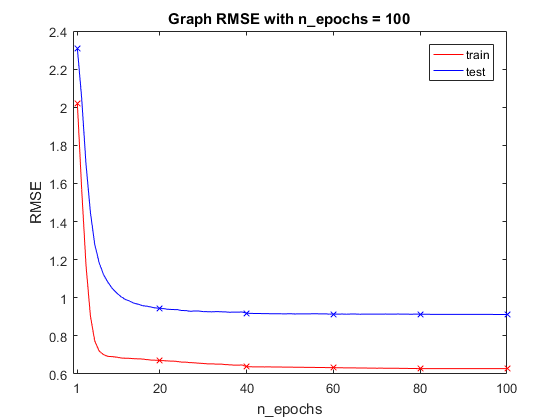
\includegraphics[scale=1]{RMSE.png}
\caption{Đồ thị RMSE cho bộ ml-100k}
\end{figure}
\end{center}
\begin{center}
\begin{figure}[h]
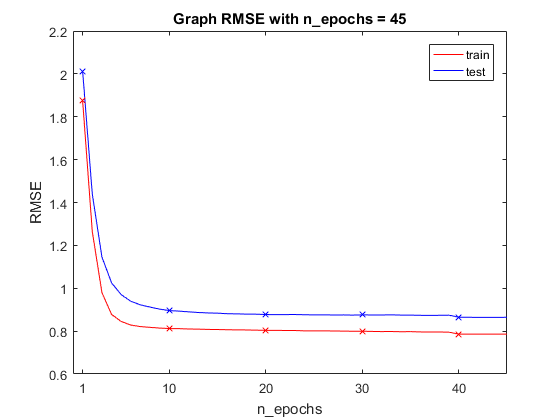
\includegraphics[scale=1]{RMSE!.png}
\caption{Đồ thị RMSE cho bộ ml-1m}
\end{figure}
\end{center}
\begin{thebibliography}{5}
\bibitem{latex}\url{http://www.mmds.org/}
\bibitem{website}Slide chapter 9 Stanford University
\bibitem{book}Mining of Massive Datasets of Jure Leskovec Stanford Univ. Anand Rajaraman Milliway Labs Jeffrey D. Ullman Stanford Univ.
\end{thebibliography}
\end{document}